\documentclass[12pt, a4paper, oneside, romanian]{article}
\usepackage{listings}
\usepackage[dvipsnames]{xcolor}
\usepackage{color}
\usepackage[utf8x]{inputenc}

% -----------------------------------------------------------------
% Pretty formatting for 2nd, 3rd etc.
\usepackage{nth}

% -----------------------------------------------------------------
% Math package
\usepackage{amsmath}

% -----------------------------------------------------------------
% Bold in math mode
\usepackage{bm}

% -----------------------------------------------------------------
% Use images
\usepackage{graphicx}
\graphicspath{ {images/} }
\usepackage{float}

% -----------------------------------------------------------------
% Settings for pretty code
\definecolor{codegray}{gray}{0.9}
\definecolor{mygray}{rgb}{0.4,0.4,0.4}
\definecolor{mygreen}{rgb}{0,0.8,0.6}
\definecolor{myorange}{rgb}{1.0,0.4,0}

% -----------------------------------------------------------------
% Settings for tables
\usepackage{array}
\usepackage{tabu}
\usepackage{makecell}

% -----------------------------------------------------------------
% For angular brackets 
\usepackage[T1]{fontenc} 

% -----------------------------------------------------------------
%          **** PAGE LAYOUT ****
% We need 1" (~72pt) margins except on the binding edge, where it is 1 1/2".
% They are a bit larger to handle lines with overfull boxes.
% 
\oddsidemargin -5mm 
\evensidemargin -5mm  %%% was 40 and 25 -dks

\marginparwidth 40bp 
\marginparsep 10bp 
\topmargin -20mm 
\leftmargin 0mm 
\rightmargin 0mm 
\textwidth 170mm
\textheight 257mm

%\topmargin -47bp        % Default margin is  73 points-- make 1/2 that
                        % plus a bit more to get page 1/2 inch down.
\headheight 10mm        % Height of box containing running head.
\headsep 5mm           % Distance between foot of head and text.
                        % headsep + headheight + topmargin ~ 72 pt
%\textheight 648bp       % Height of text (including footnotes and  %%% was 620
                        % figures, excluding running head and foot).
%\textwidth 412bp        % Give 92pt right margin;72 + extra for overfull boxes.
% disappeared from LaTeX\footheight 11bp        %    Height of box containing running foot.
\footnotesep  
\baselineskip
\footskip 15mm          %    Distance from baseline of box containing foot 
                        %    to baseline of last line of text.
\parindent 3.5ex
\parskip 1bp plus 1bp 
\setcounter{tocdepth}{3} % Put subsubsections in toc (set to 2 in
                         % report.sty). [lsc] 
\skip\footins 15pt plus3pt minus3pt % Add space between text and
                                    % footnotes.

% -----------------------------------------------------------------
% Code settings
\newcommand{\code}[1]{\colorbox{codegray}{\texttt{#1}}}

% -----------------------------------------------------------------
% Verificare ortografie romana
% aspell --lang=ro -t check ./main.tex

% -----------------------------------------------------------------
% Stuff from template ETTI
\setcounter{secnumdepth}{3}
\setcounter{tocdepth}{3}
\usepackage{babel}
\usepackage[
    bookmarks,
    bookmarksopen=true,
    pdftitle={Licenta-Laura-Flueratoru},
    linktocpage,
    hidelinks]{hyperref}

%\colorbox{codegray}{\lstinline[basicstyle=\ttfamily\color{white}]|<List>|}


\lstset{ %
    basicstyle=\footnotesize\sffamily\color{black},
    commentstyle=\color{mygray},
    captionpos=b, 	% position of the caption to bottom
    breaklines=true,	% sets automatic line breaking
    frame=single, 	% adds a frame around the text
    numbers=left,	% where to put line numbers
    numbersep=5pt,
    numberstyle=\tiny\color{mygray},
    keywordstyle=\color{mygreen},
    showspaces=false,
    showstringspaces=false,
    stringstyle=\color{myorange},
    tabsize=2
}

\begin{document}
\title{The MUSIC Flow Graph - Theory, Demo, Profiling}
\author{Fluerătoru Laura}
\date{}
\maketitle

\section{Introduction}

This report outlines the theory on which the MUSIC algorithm is founded in
Section \S\ref{sec:theory-music}, summarizes its main steps in Section
\S\ref{sec:steps-music-algo}, then Section \S\ref{sec:demo-chain} explains how
they are mapped on the flow graph for the MUSIC algorithm implemented by Ettus
Research \cite{cite:ettus-doa} that is used as a reference for the current
project.  Section \S\ref{sec:profiling-chain} shows the results of profiling the
aforementioned C++ flow graph and its actual code can be found in Section
\S\ref{sec:code-snips}.

%=============================================================================
% SECTION 2 - Steps in MUSIC Algorithm
%=============================================================================

\section{Teoria din spatele algoritmului MUSIC}
\label{sec:theory-music}

\begin{figure}[h]
    \centering
    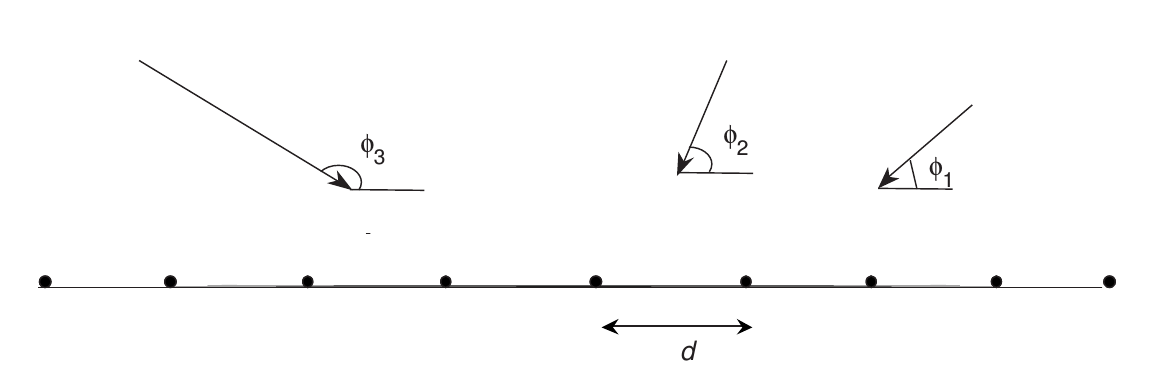
\includegraphics[width=1\textwidth]{array-for-doa}
    \caption{TODO: my own image in PS}
    \label{fig:array-for-doa}
\end{figure}


În analiza algoritmului MUSIC presupunem că plecăm de la un șir liniar de $M$
antene la care ajung $D$ semnale $s_j(t), i = \overline{1, D}$ și se dorește
estimarea unghiului de incidență $\theta_j$ măsurat față de axa $x$ în sens
trigonometric sub care ajunge fiecare semnal la șirul de antene. Presupunem că
mediul de propagare nu afectează semnificativ semnalele când acestea se propagă
de la un element din șir la altul, deci semnalul care ajunge la o antenă diferă
de cel care ajunge la o altă antenă doar printr-o întârziere $\tau$. \\

Considerăm că prima antenă se află în originea sistemului, la locația (0, 0) și
exprimăm întarzierea semnalului de la celelalte elemente din șir relativ la
semnalul care ajunge la elementul de referință. Astfel, pentru un șir liniar,
semnalul $j$ care ajunge la elementul $i = 2$ parcurge o distanță mai lungă cu
$d\,cos\theta_j$ față de primul element și, în cazul general, putem scrie
întârzierea $\tau_i$ la elementul $i$ ca
\begin{equation}
    \tau_i = \beta(i-1)d\,cos\theta_j
\end{equation}
unde $\beta = \frac{2\pi}{\lambda}$ este factorul de defazaj. \\

Aici, am presupus că defazajul semnalului depinde doar de locațiile distincte
ale elementelor șirului de antene. În realitate, antenele vor avea și ele un
răspuns dependent de directivitatea lor și de frecvență, care poate fi modelat
ca un câștig $g_i$. Obținem, astfel, vectorul director (\textit{steering
vector}) pentru un anumit unghi de incidență $\theta_j$ și frecvență $\omega$:
\begin{equation}
    \bm{a}(\omega, \theta_j) = 
	    \begin{bmatrix}
		g_1(\omega, \theta_j)e^{\tau_1(\theta_j)} \\
		... \\
		g_M(\omega, \theta_j)e^{\tau_M(\theta_j)}
	    \end{bmatrix}
\end{equation}

Prin urmare, vectorul director este dependent de răspunsul individual al
fiecărui element din șirul de antene, de geometria șirului, de frecvența
semnalului și de unghiul de incidență al acestuia. Matricea care se formează din
vectorii coloană directori pentru toate unghiurile de incidență și toate
frecvențele se numește matricea colectoare a șirului
(\textit{array manifold matrix}).
\begin{equation}
    \bm{A} = 
	    \begin{bmatrix}
		\bm{a}(\omega, \theta_1) & ... & \bm{a}(\omega, \theta_D)
	    \end{bmatrix}
\end{equation}

Dacă banda semnalului este suficient de îngustă, se poate considera, cu
aproximație, că vectorul director este independent de frecvență și că depinde doar
de unghiul de incidență. Mai mult, dacă presupunem că elementele șirului sunt
izotrope, putem elimina dependența vectorului director de câștigul $g_i,
i = \overline{1, M}$. Vom continua analiza având în vedere aceste presupuneri.\\

Putem scrie următoarea relație pentru semnalele de la intrarea fiecărei antene
din șir:
\begin{equation}
\label{eq:xasn}    
    \bm{x}(t) = 
	\begin{bmatrix}
	   \bm{a}(\theta_1) & \bm{a}(\theta_2) & ... & \bm{a}(\theta_D)
	\end{bmatrix}
	\begin{bmatrix}
	    s_1(t) \\ s_2(t) \\ ... \\ s_D(t)
	\end{bmatrix}
	+
	\begin{bmatrix}
	    n_1(t) \\ n_2(t) \\ ... \\ n_D(t)
	\end{bmatrix}
\end{equation}
\begin{equation}
\label{eq:xasn-short}
    \bm{x}(t) = \bm{A}\bm{s}(t) + \bm{n}(t)
\end{equation}

% (TODO: puțin despre cine l-a făcut + citează \cite{cite:music-schmidt})
Algoritmul MUSIC (MUltiple SIgnal Classification) face parte dintr-o clasă mai
mare de algoritmi care se bazează pe metoda subspațiilor, care ia în considerare
și zgomotul dintr-un sistem. Algoritmul oferă, în primul rând, informații despre
numărul de semnale care ajung la un șir de antene și unghiul de incidență al
acestora. Este un algoritm cu rezoluție mare, ceea ce înseamnă că poate distinge
mai ușor decât alți algoritmi două semnale care vin din direcții foarte
apropiate, dar are nevoie de o calibrare foarte precisă a șirului de antene.
Calibrarea constă în obținerea matricei colectoare a șirului de antene; în
practică, acest lucru se realizează măsurând răspunsurilor unor surse
punctiforme ale șirului la diverse unghiuri și frecvențe. Pentru explicarea
fundamentului matematic din spatele algoritmului MUSIC s-a folosit ca referință
lucrarea \cite{cite:doa-1996}, în care este tratat pe larg subiectul estimării
unghiurilor de incidență folosind șiruri de antene.\\

În ecuația \eqref{eq:xasn}, vectorul $\bm{x}$ al semnalelor de la intrarea
antenelor din șir și vectorii directori $\bm{a}(\theta_j), j = \overline{1, D}$
pot fi priviți ca vectori într-un spațiu cu M dimensiuni, ceea ce înseamnă că
$\bm{x}$ poate fi scris ca o combinație liniară între vectorii directori, unde $s_j,
j = \overline{1, D}$ sunt coeficienții combinațiilor. \\

Se poate calcula matricea de covarianță a intrării
\begin{equation}
    \bm{R}_{xx} = E[\bm{xx}^H] = \bm{A}E[\bm{ss}^H]\bm{A}^H + E[\bm{nn}^H]
\end{equation}
\begin{equation}
    \bm{R}_{xx} = \bm{A}\bm{R}_{ss}\bm{A}^H + \sigma^2_{zg}\bm{I}
\end{equation}

S-a notat $\bm{R}_{ss} = E[\bm{ss}^H]$ matricea de corelație a semnalului $s$.
Se observă două proprietăți importante:
\begin{itemize}
    \item Vectorii directori sunt liniar independenți, ceea ce înseamnă că
    matricea $\bm{A}$ este de rang maxim.
    \item $\bm{R}_{ss}$ este o matrice nesingulară dacă semnalele incidente sunt
    cel mult parțial necorelate. Dacă ar fi corelate, atunci cel puțin una
    dintre liniile/coloanele sale ar putea fi scrisă ca o combinație liniară a
    altor linii/coloane, ceea ce ar însemna că matricea ar avea determinantul
    egal cu 0, deci ar fi singulară și nu am mai putea folosi algoritmul.
\end{itemize}

Din aceste două proprietăți rezultă că, dacă $M < D$, atunci matricea
$\bm{A}\bm{R}_{ss}\bm{A}^H$ este pozitiv semidefinită, având rangul D. Din
această proprietate, se poate demonstra faptul că $M - D$ dintre valorile
proprii ale matricei trebuie să fie nule. Folosind relația
\eqref{eq:xasn-short}, reiese că atunci când $M - D$ dintre valorile proprii ale
matricei $\bm{A}\bm{R}_{ss}\bm{A}^H$ sunt nule, cele mai mici valori proprii ale
matricei $\bm{R}_{xx}$ vor fi egale cu puterea zgomotului $\sigma_{zg}^2$. Dacă
notăm $\lambda_i, i = \overline{1, M}$ valorile proprii ale matricei
$\bm{R}_{xx}$, atunci
\begin{equation}
    \lambda_{D+1} = \lambda_{D+2} = ... = \lambda_M = \lambda_{min} = \sigma_{zg}^2
\end{equation}

În realitate, însă, nu se va îndeplini egalitatea, deoarece folosim
pentru estimare doar un număr finit de eșantioane, dar valorile vor fi,
într-adevăr, foarte apropiate. Dacă notăm $K$ multiplicitatea celei mai mici
valori proprii a matricei $\bm{R}_{xx}$, atunci, știind că $M = D + K$, putem
estima numărul semnalelor care ajung la șirul de antene
\begin{equation}
    \hat{D} = M - K
\end{equation}

Din definițiile valorilor proprii și a vectorilor proprii \cite{cite:gol-89}, vectorii
proprii $\bm{v}_i, i = \overline{1, M}$ corespunzători celor mai mici valori
proprii trebuie să satisfacă egalitatea
\begin{equation}
    \bm{R}_{xx}\bm{v}_i = \sigma_{zg}^2\bm{v}_i, \quad i = \overline{D+1, M}
\end{equation}
Folosind ecuația \eqref{eq:xasn-short}, înseamnă că
\begin{equation}
    \bm{A}\bm{R}_{ss}\bm{A}^H\bm{v}_i = 0, \quad i = \overline{D+1, M}
\end{equation}
Știind că $\bm{A}$ este de rang maxim și că $\bm{R}_{ss}$ este nesingulară,
atunci
\begin{equation}
    \bm{A}^H\bm{v}_i = 0, \quad i = \overline{D+1, M}
\end{equation}
ceea ce este echivalent cu a spune că vectorii coloană ai matricei $\bm{A}$,
adică vectorii directori, sunt perpendiculari pe vectorii proprii ai matricei
$\bm{R}_{xx}$. 
\begin{equation}
    \begin{bmatrix}
	\bm{a}(\theta_1) & \bm{a}(\theta_2) & ... & \bm{a}(\theta_D)
    \end{bmatrix}
    \bot
    \begin{bmatrix}
	\bm{v}_{D+1} & \bm{v}_{D+2} & ... & \bm{v}_M
    \end{bmatrix}
\end{equation}

Recapitulând, avem două subspații ortogonale: cel al semnalelor și cel al
zgomotului. Vectorii directori ai șirului de antene aparțin subspațiului
semnalelor și, așadar, sunt perpendiculari pe subspațiul zgomotului, iar
vectorii proprii ai matricei de covarianță $\bm{R}_{xx}$ pot aparține oricăruia
dintre cele două subspații. Prin urmare, putem să căutăm printre vectorii
directori pe aceia care sunt ortogonali pe subspațiul zgomotului, în care se vor
afla o parte din vectorii proprii ai matricei de covarianță, și să determinăm
unghiurile de incidență $\theta_j$.

Se calculează spectrul MUSIC folosind una dintre următoarele două forumle:
\begin{equation}
    P_{MUSIC}(\theta) =
        \frac{\bm{a}^H(\theta)\bm{a}(\theta)}
             {\bm{a}^H(\theta)\bm{V}_N\bm{V}_N^H\bm{a}(\theta)} \\
\end{equation}
\begin{equation}
    P_{MUSIC}(\theta) =
        \frac{1}
             {\bm{a}^H(\theta)\bm{V}_N\bm{V}_N^H\bm{a}(\theta)} \\
\label{eq:music-spectrum}
\end{equation}
\begin{equation}
    \bm{V}_N = \begin{bmatrix}v_{D+1}, & ..., & v_M \end{bmatrix}
\end{equation}
și, în cazul în care vectorii directori sunt perpendiculari pe vectorii proprii,
numitorul va fi minim, ceea ce va conduce la apariția unor vârfuri în spectru.
Cunoaștem numărul de semnale estimat $\hat{D}$, deci cele $\hat{D}$
vârfuri din spectru corespund unghiurilor de incidență căutate.

%=============================================================================
% SECTION 2 - Steps in MUSIC Algorithm
%=============================================================================

\section{Outline of the MUSIC Algorithm}
\label{sec:steps-music-algo}
The theory behind the MUSIC algorithm discussed in section
\S\ref{sec:theory-music} can be summarized in some elementary steps. We remind
that M is the number of elements in the antenna array and D is the number of
incoming signals at each element.

\subsection*{Step 1}
\label{ssec:step1}
Knowing the signal $x_i$ arriving at the element number \textit{i} of the
antenna array, the input covariance matrix can be computed:
\begin{equation}
    \bm{R}_{xx} = E[\bm{xx}^H]
\end{equation}
\begin{equation}
    x = \begin{bmatrix}x_1 & x_2 & ... & x_M \end{bmatrix} \\
\end{equation}

\subsection*{Step 2}
\label{ssec:step2}
Estimate the number of signals arriving at each element of the array. In order
to do this, we need to compute the eigenvalues of $R_{xx}$ and, from the
multiplicity $K$ of the smallest eigenvalue, we estimate the number of signals
as follows:
\begin{equation}
    \hat{D} = M - K
\end{equation}

\subsection*{Step 3}
\label{ssec:step3}
Compute the MUSIC spatial spectrum using
\begin{equation}
    P_{MUSIC}(\theta) =
        \frac{\bm{a}^H(\theta)\bm{a}(\theta)}
             {\bm{a}^H(\theta)\bm{V}_N\bm{V}_N^H\bm{a}(\theta)} \\
\end{equation}
\begin{equation}
    \bm{V}_N = \begin{bmatrix}v_{D+1}, & ..., & v_M \end{bmatrix}
\end{equation}

\subsection*{Step 4}
\label{ssec:step4}
Find the peaks of the estimated MUSIC spectrum which give us direction of
arrival for the $\hat{D}$ signals.

%=============================================================================
% SECTION 3 - The Demo Chain
%=============================================================================

% TODO maybe change title...
\section{The Demo Chain}
\label{sec:demo-chain}
In order to assess the performance of the MUSIC algorithm, an implementation
created by Ettus Research \cite{cite:ettus-doa} has been used. They provide an
application which proves the phase synchronization capability of their TwinRX
daughtercards, inside the GNU Radio framework. Figure \ref{fig:grc-fg} shows the
flow graph created with the GNU Radio Companion. \\

\begin{figure}[h]
    \centering
    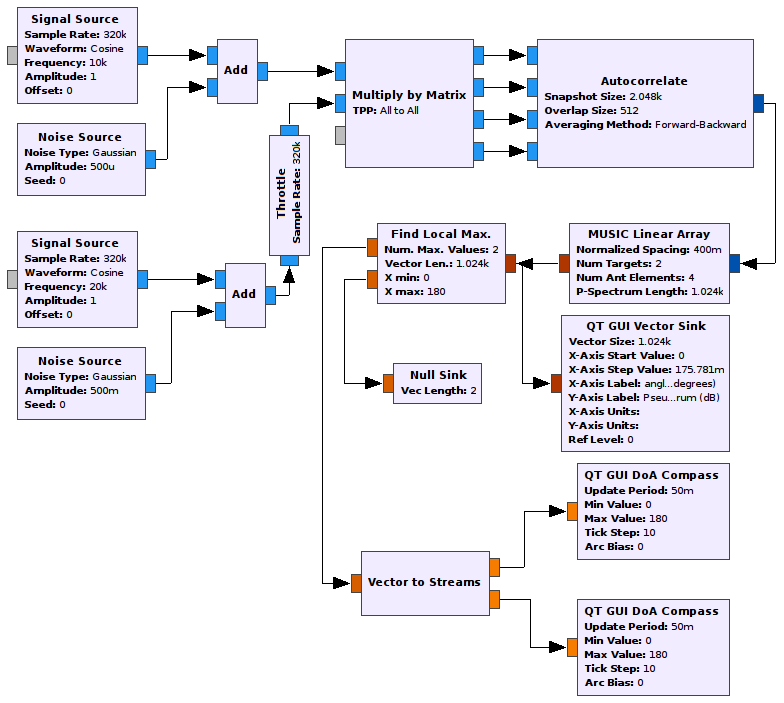
\includegraphics[width=\textwidth]{graph_doa}
    \caption{The flow graph used for the MUSIC algorithm}
    \label{fig:grc-fg}
\end{figure}


To explain the functionality of the graph, we need to define a set of
parameteres used in various block. The names of the parameters do not
necessarily reflect the actual names of the variables used in the code, but make
it easier to identify the parameters of interest. Also, some parameters are also
denoted by a shorter name, to make notations easier where it applies.
\begin{itemize}
  \item \code{sample\_rate} The rate at which the input signal is sampled
  \item \code{tone\_freq\_i} The frequency of the $i^{th}$ input signal
  \item \code{norm\_spacing} The normalised distance between the elements of the
  antenna array
  \item \code{num\_targets} The number of input signals, also denoted by N
  \item \code{num\_array\_elements} The number of elements in the antenna array,
  also denoted by M
  \item \code{p\_spectrum\_length} The length of the computed MUSIC spectrum
  \item \code{snapshot\_size} The number of samples used in computing the
  autocorrelation, also denoted by K
  \item \code{overlap\_size} The number of samples that overlap when computing
  successive values of the autocorrelation
\end{itemize}

\subsection{The input data}
This configuration uses two signal sources ($D = 2$) which generate cosines of
frequencies 10 kHz and 20 kHz, over which we add Gaussian noise, and an antenna
array with four elements ($M = 4$). The \textbf{Throttle} block is
used to limit the data throughput to the frequency of the input signal's
frequency, as it would behave in the case of a real signal arriving at an
antenna.

\subsection{The Multiply by Matrix block}
This block is used to simulate the way signals arrive at the antenna array, by
multiplying the array manifold matrix with an array which consists of samples of
the incoming signals. The general behaviour of the block is that if $\bm{A}$ is
the matrix that is given as a parameter to the block, of size M by N, and
$\bm{X}_N$ is a column array built from the $N$ inputs given to the block, then
the result of the multiplication is
\begin{equation}
\bm{Y}_M = \bm{A}\bm{X}_N,
\end{equation}
where $\bm{Y}_M$ is an column array constructed from the outputs of the block.
Thus, the block should have a number of N inputs and M outputs. \\

The array manifold matrix takes into account the angles of arrival and the
normalised distance between the elements of the array. The normalised spacing is
the distance between the antenna elements divided by the wavelength of the
carrier. According to \cite{cite:ettus-doa}, the normalised spacing should be at
most half of the center wavelength of the signal, otherwise aliasing could
interfere with the angle resolution performance of the MUSIC algorithm. \\

In our case, the array manifold matrix is:
\begin{displaymath}
    \begin{bmatrix}
        \bm{a}(\theta_1) & \bm{a}(\theta_2)
    \end{bmatrix}
\end{displaymath}
where $\bm{a}(\theta_i)$ is the steering vector corresponding to the angle of
arrival of the $i^{th}$ signal. The outputs of the \textbf{Multiply by Matrix}
block represent the sum of the signals that arrive at different angles at each
element of the antenna array.

% TODO find out why in the algorithm they use the autocorrelation rather then
% the autocovariance. it's just a normalization missing, but maybe it's
% important
\subsection{The Autocorrelate block}
The following block, \textbf{Autocorrelate}, corresponds to the step
\S1 of the MUSIC algorithm, although it actually computes an estimate of the
autocorrelation of the signal in the form of a sample correlation matrix. This
method implies collecting a sample over a snapshot time of the signal that
arrives at each element of the antenna array. Thus, an M by 1 array is formed,
denoted $x(k)$, and the sample correlation matrix is computed as follows:
\begin{equation}
C_x = \frac{1}{K}\sum_{k=1}^{K}\bm{x}(k)\bm{x}^H(k).
\end{equation}

Another method of computing the sample correlation matrix is collecting a number
of samples over a snapshot period denoted K, forming the matrix $\bm{X_K}$ of
dimensions N by K, which leads to the following formula:
\begin{equation}
C_x = \frac{1}{K}\bm{X_K}\bm{X_K}^H.
\label{eq:autocorr-first-part}
\end{equation}

In \cite{cite:FB-Averaging} it has been suggested that an additional step
consisting of a Forward-Backward Averaging of the sample correlation matrix will
increase the performance of the DoA estimation, so the computation can be
adjusted as such:
\begin{equation}
C_x = \frac{1}{2K}\bm{X_K}\bm{X_K}^H + \frac{1}{2K}\bm{J}\bm{X_K}^*\bm{X_K}^T\bm{J},
\end{equation}
where J is a reflection matrix (elements on the cross-diagonal are equal to 1
and the rest are 0). \\

The parameters of the \textbf{Autocorrelate} block are:
\begin{itemize}
    \item Snapshot size, previously denoted as K, representing the number of
    input samples used in computing the correlation matrix for an output item
    \item Overlap size, the number of samples that overlap in the computation
    for an output item to the next
    \item Averaging method, which can be either Forward-Backward or the standard
    Forward method
\end{itemize}

\subsection{The MUSIC Linear Array block}
In this application, we assume that we know the number of targets, so we do not
need a separate block to perform step \S2. Therefore we proceed directly to the
\textbf{MUSIC Linear Array} block, which computes the MUSIC spatial spectrum
from the step \S3. \\

In the constructor of the block, an array manifold vector is generated, which
uses a span of the possible angles between 0 and 180 degrees, with a resolution
of \code{1/d\_spectrum\_length}. The way the algorithm works, the closer an angle used
in generating the array manifold vector is to the actual angle of arrival, the
closer the MUSIC spectrum is to 0. In theory, when they coincide, the MUSIC
spectrum will reach 0. Therefore, for each input item a number of
\code{d\_spectrum\_length} values of the MUSIC spectrum have to be computed. \\

To compute the MUSIC spectrum, the block takes as input the result of the
autocorellation, on which an EigenValue Decomposition (EVD) is performed, and
then the desired spectrum is computed according to forumla
\eqref{eq:music-spectrum}. The block takes as parameters the number of targets,
the number elements in the antenna array and the normalised distance between
them, and also the spectrum length. \\

% TODO: why they take only the real part of Q_temp

\subsection{The Find Local Max block}
In order for the application to find the precise values of the angles of
arrival, a further block named \textbf{Find Local Max.} is needed, which solves
the step \S4 of the algorithm. The block outputs the coordinates (that is, the
angle) at which the peaks in the spectrum are found and looks precisely for $D$
such maximums. The block also gives information about the amplitude of the
spectrum at the given locations, but since they are of no importance for this
application, they are directed towards a \textbf{Null Sink}.

\subsection{Visualising the results}
We can either visualise the spectrum immediately after the \textbf{MUSIC Linear
Array} block, such as in Figure \ref{fig:doa-sp}, and form a good idea about the
estimated angle of arrival with the \textbf{QT GUI Vector Sink} block or, using
the \textbf{QT GUI DoA Compass} widget, we can see the estimated angle of
arrival for the two signals after we found the peaks in the spectrum. One
example of such an output for one of the signals can be found in Figure
\ref{fig:doa-compass}. Using two sliders, we can change the angle of arrivals in
real time and observe how the algorithm is adapting to the changes.

\begin{figure}[H]
    \centering
    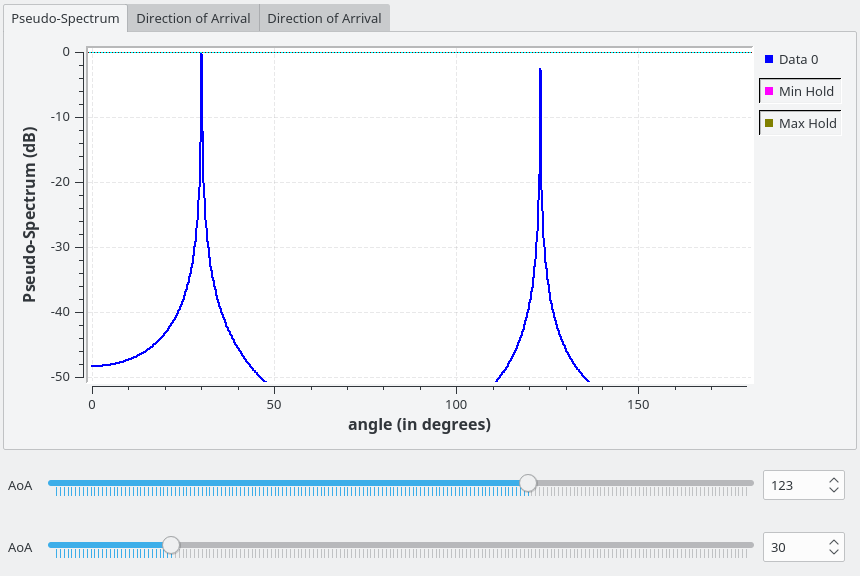
\includegraphics[width=0.75\textwidth]{grc-doa-spectrum}
    \caption{The MUSIC spectrum}
    \label{fig:doa-sp}
\end{figure}
\begin{figure}[H]
    \centering
    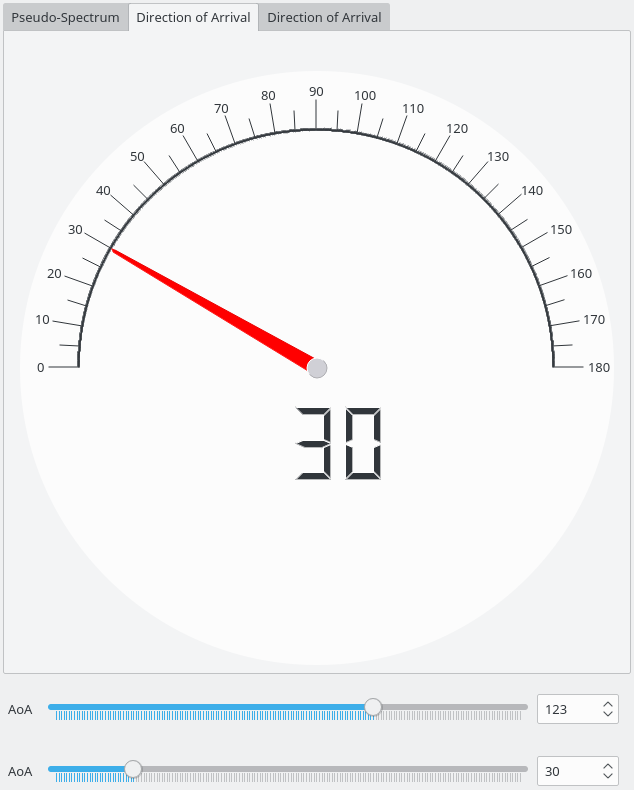
\includegraphics[width=0.4\textwidth]{grc-doa-compass}
    \caption{The estimated angle of arrival for one signal}
    \label{fig:doa-compass}
\end{figure}

%=============================================================================
% SECTION 4 - The Profiling Chain
%=============================================================================

% TODO maybe change title...
\section{The Profiling Chain}
\label{sec:profiling-chain}
% TODO is it important - for the profiling - to change the AoA to see the
% performance? if not, how do i motivate this?
\subsection{Profile Methodology}

The GNU Radio Companion generates a Python script based on the flow graph
created in the graphic interface. The Python script then uses SWIG
\cite{cite:swig}, a tool that enables it to access the modules written in C++
and execute the flow graph.  Because of this intermediary step, the profiling
performed on the script is not very conclusive, since functions needed in the
wrapping process that are not directly related to the algorithm itself end up
consuming much of the execution time. For this reason, the preferred solution
was to create a C++ program that creates a flow graph similar to the initial
one, which also eliminates the dependency on a visual interface. \\

In this test program all the Qt blocks previously used are eliminated and, where
necessary, they are replaced with \textbf{Null Sink} blocks, which simply
discard the data feeding them, so that there are no time consuming I/O
operations. Additionally, the \textbf{Throttle} block is also discarded because
we want to profile the program when it runs at full speed. \\

After the program starts the flow graph, it creates a new thread and, after it
sleeps for 2 seconds (a period of time that can be adjusted), it calls for the
flow graph to stop its execution, otherwise it would run indefinitely. The full
code of the C++ flow graph and its Makefile can be found in Section
\ref{sec:code-snips}, in Listing \ref{lst:cpp-fg} and Listing
\ref{lst:cpp-fg-makefile}, respectively. \\

% TODO the hardware events vary with the processor - if we also profile it on
% ARM we should also be sure that we are comparing quite the same things
For profiling the processing chain, both \textbf{perf} \cite{cite:perf} and
\textbf{callgrind} \cite{cite:callgrind} have been used. \textbf{perf} is a
powerful tool for measuring a large set of hardware events, which also displays
assembly code for functions of interests, which can be helpful when wanting to
target micro-optimizations.  With \textbf{callgrind}, on the other hand, there
is the option of using the visual interface \textbf{kcachegrind}
\cite{cite:kcachegrind} for an easier tracing of the call graph. In this case,
the percentage of time spent in different functions is of interest, and both of
the profiling tools gave similar results. \\

Using \textbf{perf}, we can obtain how many cycles are spent in each function by using
the command:
\begin{lstlisting}[language=bash]
perf record -e cycles ./run_MUSIC_profile
\end{lstlisting}

If we want to view the call graph, we can instead use:
\begin{lstlisting}[language=bash]
perf record --call-graph lbr ./run_MUSIC_profile
\end{lstlisting}

Profiling the code with \textbf{callgrind} can be done with the following
command:
\begin{lstlisting}[language=bash]
valgrind --tool=callgrind ./run_MUSIC_profile
\end{lstlisting}

Since the results with both of the profilers are similar, only the ones obtained
with \textbf{perf} will be outlined. Of particular interest is the case when the
maximum level of optimization is being used, but since the call succession
cannot be observed very well in this case, another analysis with the lowest
level of optimization and debug symbols has been performed. The profiling flow
graph uses functions from the \textit{gr-doa} library of Ettus Research, as well
as from \textit{Armadillo} \cite{cite:armadillo}, a C++ library for linear
algebra, which was compiled from sources, as the latest version needed cannot be
found yet in the official repositories. The processing blocks rely internally
heavily on functions implemented in \textit{Armadillo} which may end up being
computing intensive, so when compiling the profiling chain with level 0 of
optimization, we have to make sure that both of the libraries are compiled in
the same way in order to see the hot spots of the processing chain.

\subsection{Profile results}

Using the maximum level of optimization, the most important profiling results
(for the functions which consume more than 2\% of the execution time) are
presented in Table \ref{tab:prof-o3}. \\

%=============================================================================
% Profiling table
%=============================================================================
\begin{table}[!htb]
\begin{center}
 \begin{tabular}{||c c c||} 
 \hline
 Overhead  & Command & Symbol \\ [0.5ex] 
 \hline\hline
 49,14\% 
 &
 find\_local\_max6
 &
 \makecell{arma::glue\_hist::apply\_noalias<unsigned int>}
 \\ 
 
 \hline
 13,73\%
 &
 autocorrelate4
 &
 \makecell{cgemm\_}
 \\
 
  \hline
 10,51\%
 &
 MUSIC\_lin\_array
 &
 \makecell{cgemm\_}
 \\
 
 \hline
 3,63\%
 &
 multiply\_matrix
 &
 \makecell{\_\_mulsc3}
 \\

  \hline
 3,56\%
 &
 MUSIC\_lin\_array
 &
 \makecell{cgemv\_}
 \\

  \hline
 3,06\%
 &
 MUSIC\_lin\_array
 &
 \makecell{gr::doa::MUSIC\_lin\_array\_impl::work}
 \\

  \hline
 2,33\%
 &
 MUSIC\_lin\_array
 &
 \makecell{\_\_logf\_finite}
 \\

  \hline
 2,08\%
 &
 multiply\_matrix  
 &
 \makecell{gr::blocks::multiply\_matrix\_cc\_impl::work}
 \\ [1ex] 
 \hline
\end{tabular}
\end{center}
\caption{Profiling Results With -O3}\label{tab:prof-o3}
\end{table}


According to the documentation of the tool, \textit{Overhead} is the percentage
of time spent in a particular function, \textit{Command} is the name of the task
that can be read via \code{/proc/<pid>/comm}, and \textit{Symbol} is the name of
the function executed at the moment of sampling. \\

Table \ref{tab:prof-o0} presents the output produced by \code{perf report} when
the libraries and the project are compiled with the lowest level of
optimization. \\

%=============================================================================
% Profiling table
%=============================================================================
\begin{table}[H]
\begin{center}
 \begin{tabular}{||c c c||} 
 \hline
 Overhead  & Command & Symbol \\ [0.5ex] 
 \hline\hline
 49,87\% 
 &
 find\_local\_max6
 &
 \makecell{arma::glue\_hist::apply\_noalias<unsigned int>}
 \\ 
 
 \hline
 6,36\%
 &
 autocorrelate4
 &
 \makecell{cgemm\_}
 \\
 
 \hline
 4,81\%  
 &
 autocorrelate4
 &
 \makecell{std::conj<float>}
 \\
 
 \hline
 4,66\%
 &
 MUSIC\_lin\_array
 &
 \makecell{std::complex<float>::complex}
 \\
 
 \hline
 3,38\%
 &
 MUSIC\_lin\_array
 &
 \makecell{cgemm\_}
 \\

 \hline
 2,46\%
 &
 autocorrelate
 &
 \makecell{arma::eop\_core<arma::eop\_conj>::apply \\
 <arma::Mat<std::complex<float> >, \\
 arma::Mat<std::complex<float> > >}
 \\

 \hline
 1,82\%
 &
 MUSIC\_lin\_array
 &
 \makecell{arma::Mat<std::complex<float> >:: \\
 init\_warm}
 \\

 \hline
 1,57\%
 &
 autocorrelate4
 &
 \makecell{arma::op\_strans::apply\_mat\_noalias \\
 <std::complex<float>,\\
 arma::Mat<std::complex<float> > >}
 \\

 \hline
 1,54\%
 &
 multiply\_matrix  
 &
 \_\_mulsc3
 \\

 \hline
 1,49\%
 &
 MUSIC\_lin\_array
 &
 cgemv\_
 \\ [1ex] 
 \hline
\end{tabular}
\end{center}
\caption{Profiling Results With -O0}\label{tab:prof-o0}
\end{table}


With further investigation, it is found that the most time consuming function is
\code{arma::glue\_hist::} \code{apply\_noalias<unsigned int>}, a function from
the \textit{Armadillo library} which is called from the function
\code{find\_local\_max}, responsible for finding the peaks in the MUSIC
spectrum. More precisely, the function is called from the \code{hist} functions
which is used in Listing \ref{lst:find-local-max}. \\

\begin{minipage}{\linewidth}
\lstset{
	language=C++,
	directivestyle={\color{black}},
	emph={int,char,double,float,unsigned},
	emphstyle={\color{RoyalBlue}}
    }		
\begin{lstlisting}[
	firstnumber=105,
	caption={Computationally Intensive Part in find\_local\_max},
	label={lst:find-local-max}
    ]
// finding all peak locations by computing
// second-order difference of
// sign of first-order difference
uvec indx2 = find(diff(sign_fod_in_vec) == -2)+1;

uvec indx3;
uvec indx3_unique;
uvec hist_indx3;
uvec all_pk_indxs;
if (!indx2.is_empty())
{
    // finding set-intersection between indx1 and indx2
    // in order to identify local peaks
    indx3 = join_vert(indx1, indx2);
    indx3_unique = unique(indx3);
    hist_indx3 = hist(indx3, indx3_unique);

    all_pk_indxs = indx1(find(hist_indx3 == 2));
}
\end{lstlisting}
\end{minipage}

TODO: explain what that part isn't necessary in most of the cases and which are
those \\

By eliminating that processing overhead where it is not necessary, we obtain the
new profiling results in Table \ref{tab:prof-remove}, where only the functions
that make up more than 5\% of the execution time are presented. 

%=============================================================================
% Profiling table
%=============================================================================
\begin{table}[H]
\begin{center}
 \begin{tabular}{||c c c||} 
 \hline
 Overhead  & Command & Symbol \\ [0.5ex] 
 \hline\hline
 12,73\% 
 &
 autocorrelate8
 &
 \makecell{cgemm\_}
 \\ 
 
 \hline
 11,50\%
 &
 MUSIC\_lin\_array
 &
 \makecell{cgemm\_}
 \\
 
 \hline
 7,93\%  
 &
 noise\_source\_c3
 &
 \makecell{\_\_ieee754\_log\_avx}
 \\
 
 \hline
 7,89\%  
 &
 noise\_source\_c4
 &
 \makecell{\_\_ieee754\_log\_avx}
 \\
 
 \hline
 6,98\%  
 &
 noise\_source\_c3
 &
 \makecell{gr::random::ran1}
 \\
 
 \hline
 6,42\%  
 &
 noise\_source\_c4
 &
 \makecell{gr::random::gasdev}
 \\
 
 \hline
 6,09\%  
 &
 noise\_source\_c4
 &
 \makecell{gr::random::ran1}
 \\
 
 \hline
 5,32\%  
 &
 noise\_source\_c3
 &
 \makecell{gr::random::gasdev}
 \\
 
 \hline
 5,32\%  
 &
 MUSIC\_lin\_array
 &
 \makecell{gr::doa::MUSIC\_lin\_array\_impl::work}
 
 \\ [1ex] 
 \hline
\end{tabular}
\end{center}
\caption{Profiling Results After Corrections}\label{tab:prof-remove}
\end{table}


Out of them, the ones related to the noise source are not of interest, since
they are relevant only for the simulation process, and we will therefore focus
only on the first two results. \\

Using the profiling tools, we find out that the hotspot in the \textbf{MUSIC
Linear Array} block is the computation of the MUSIC spectrum using
\eqref{eq:music-spectrum}, which can be found in Listing \ref{lst:hot-music}, on
line 136. \\

\begin{minipage}{\linewidth}
\lstset{
	language=C++,
	directivestyle={\color{black}},
	emph={int,char,double,float,unsigned},
	emphstyle={\color{RoyalBlue}}
    }		
\begin{lstlisting}[
	firstnumber=134,
	caption={Computationally Intensive Part in the MUSIC Linear Array block},
	label={lst:hot-music}
    ]
for (int ii = 0; ii < d_pspectrum_len; ii++)
{
  Q_temp = as_scalar(d_vii_matrix_trans.row(ii) * U_N_sq * d_vii_matrix.col(ii));
  out_vec(ii) = 1.0 / Q_temp.real();
}
\end{lstlisting}
\end{minipage}

As far as the autocorrelation is concerned, the computationally intensive part
is done in the first part of the calculation of the autocorrelation,
corresponding to formula \eqref{eq:autocorr-first-part}. 
Listing \ref{lst:hot-autocorrelation} depicts the part of the code
that performs this specific function. The \code{d\_input\_matrix} is already
stored in a transposed form, which explains the differences between the formula
and the code. \\

\begin{minipage}{\linewidth}
\lstset{
	language=C++,
	directivestyle={\color{black}},
	emph={int,char,double,float,unsigned},
	emphstyle={\color{RoyalBlue}}
    }		
\begin{lstlisting}[
	firstnumber=105,
	caption={Computationally Intensive Part in autocorrelate},
	label={lst:hot-autocorrelation}
    ]
out_matrix =
    (1.0 / d_snapshot_size) * d_input_matrix.st() * conj(d_input_matrix);
\end{lstlisting}
\end{minipage}

\subsubsection{Profile results on the Xilinx ZedBoard Zynq-7000 ARM/FPGA SoC
Development Board}

% TODO: how many details about the techincal specifications?
The ConnexArray SIMD processor that will be used for offloading certain parts of
the MUSIC algorithm is implemented on the FPGA on a Zedboard Zynq-7000
development board \cite{cite:zedboard}. Therefore, we are also interested in
profiling the application on the processor on the board, which is a Dual-Core
ARM Cortex A9 processor. The time ratio spent in the main functions is similar
to the previous results, the only difference lying in the number of samples
processed in the same amount of time (in this case, 30 seconds) during which the
chain is running - 5664 compared with 69879 on the Intel processor. \\

Table \ref{tab:prof-zedboard} presents the profiling results on the Dual-Core
ARM Cortex A9 processor, leaving only the results that end up consuming more
than 5\% of the processing time.

%=============================================================================
% Profiling table
%=============================================================================
\begin{table}[H]
\begin{center}
 \begin{tabular}{||c c c||} 
 \hline
 Overhead  & Command & Symbol \\ [0.5ex] 
 \hline\hline
 15,19\% 
 &
 autocorrelate8
 &
 \makecell{cgemm\_}
 \\ 
 
 \hline
 10,73\%
 &
 MUSIC\_lin\_array
 &
 \makecell{cgemm\_}
 \\
 
 \hline
 5,73\%  
 &
 noise\_source\_c4
 &
 \makecell{\_\_logf\_finite}
 \\
 
 \hline
 5,62\%  
 &
 noise\_source\_c3
 &
 \makecell{\_\_logf\_finite}

 \\ [1ex] 
 \hline
\end{tabular}
\end{center}
\caption{Profiling Results After Corrections on ARM Cortex A9}\label{tab:prof-zedboard}
\end{table}




%============================================================================
% CODE SNIPPETS
%============================================================================

\newpage
\section{Code snippets}
\label{sec:code-snips}

	\subsection{The C++ Flow Graph Used for Profiling}
	\label{ssec:code-profiling}
		\lstset{
		    language=C++,
		    directivestyle={\color{black}},
		    emph={int,char,double,float,unsigned},
		    emphstyle={\color{RoyalBlue}}
		}		
		\begin{lstlisting}[
		    caption={The C++ Flow Graph Used for Profiling},
		    label={lst:cpp-fg}
		]
#include <gnuradio/top_block.h>
#include <gnuradio/analog/sig_source_c.h>
#include <gnuradio/blocks/multiply_matrix_cc.h>
#include <gnuradio/blocks/null_sink.h>
#include <gnuradio/blocks/vector_to_streams.h>
#include <gnuradio/blocks/file_sink.h>
#include <gnuradio/blocks/vector_sink_f.h>
#include <gnuradio/blocks/vector_sink_c.h>
#include <gnuradio/gr_complex.h>

#include <doa/autocorrelate.h>
#include <doa/MUSIC_lin_array.h>
#include <doa/find_local_max.h>

#include <cmath>
#include <complex>
#include <chrono>
#include <thread>
#include <boost/math/constants/constants.hpp>

struct input_variables
{
    double sample_rate;
    double tone_freq1;
    double tone_freq2;
    float norm_spacing;
    int num_targets;
    int num_array_elements;
    int p_spectrum_length;
    int snapshot_size;
    int overlap_size;
};


int main(int argc, char **argv)
{
    using namespace std::complex_literals;

    gr::top_block_sptr fg = gr::make_top_block("run_MUSIC");

    const float pi = boost::math::constants::pi<float>();

    /*=============================================
     * Variables
     *============================================*/
    struct input_variables in_vars = {
        320000, // sample_rate
        10000,  // tone_freq1
        20000,  // tone_freq2
        0.4,    // norm_spacing
        2,      // num_targets
        4,      // num_array_elements
        1024,   // p_spectrum_length
        2048,   // snapshot_size
        512     // overlap_size
    };
    int theta0_deg = 50;
    int theta1_deg = 140;
    float theta0 = pi * theta0_deg / 180;
    float theta1 = pi * theta1_deg / 180;
    
    std::vector<gr_complex> amv0(in_vars.num_array_elements);
    std::vector<gr_complex> amv1(in_vars.num_array_elements);
    std::vector<std::vector<gr_complex>> array_manifold_matrix(
        in_vars.num_array_elements,
        std::vector<gr_complex>(in_vars.num_targets)
    );
    float ant_loc_val;
    
    if (in_vars.num_array_elements % 2 == 1) {
        ant_loc_val = (float)in_vars.num_array_elements / 2;
    } else {
        ant_loc_val = (float)in_vars.num_array_elements/2 - 0.5;
    }

    // can't multiply by an integer (2) when we have -1if
    float temp_norm_spacing = in_vars.norm_spacing * 2;
    for (int i = 0; i < in_vars.num_array_elements; i++) {
        amv0[i] = std::exp(-1if * temp_norm_spacing * pi * 
			    ant_loc_val * cosf(theta0));
        amv1[i] = std::exp(-1if * temp_norm_spacing * pi *
			    ant_loc_val * cosf(theta1));
        array_manifold_matrix[i][0] = amv0[i];
        array_manifold_matrix[i][1] = amv1[i];

        ant_loc_val--;
    }
    
    /*=============================================
     * Blocks
     *============================================*/
    
    gr::analog::sig_source_c::sptr sig_src1 = 
        gr::analog::sig_source_c::make(
            in_vars.sample_rate,
            gr::analog::GR_COS_WAVE, // waveform used
            in_vars.tone_freq1,     // wave frequency
            1,                      // amplitude
            0                       // offset
        );
    
    gr::analog::sig_source_c::sptr sig_src2 = 
        gr::analog::sig_source_c::make(
            in_vars.sample_rate,
            gr::analog::GR_COS_WAVE, // waveform used
            in_vars.tone_freq2,     // wave frequency
            1,                      // amplitude
            0                       // offset
        );

    gr::blocks::multiply_matrix_cc::sptr mult_by_matrix1 = 
        gr::blocks::multiply_matrix_cc::make(
            array_manifold_matrix,
            gr::block::TPP_ALL_TO_ALL
        );

    gr::doa::autocorrelate::sptr autocorr1 = 
        gr::doa::autocorrelate::make(
            in_vars.num_array_elements,
            in_vars.snapshot_size,
            in_vars.overlap_size,
            1 
        );
    
    gr::doa::MUSIC_lin_array::sptr music_lin_array1 =
        gr::doa::MUSIC_lin_array::make(
            in_vars.norm_spacing,
            in_vars.num_targets,
            in_vars.num_array_elements,
            in_vars.p_spectrum_length
        );

    gr::doa::find_local_max::sptr find_local_max1 = 
        gr::doa::find_local_max::make(
            in_vars.num_targets,
            in_vars.p_spectrum_length,
            0.0, // min value of index vector
            180.0 // max value of index vector
        );

    // Null sink for locations
    gr::blocks::null_sink::sptr null_sink1 = 
        gr::blocks::null_sink::make(
            sizeof(float) * in_vars.num_targets // item size
        );

#ifdef PROFILE_GR_DOA    
    // Null sink for directions of arrival ---> for profiling
    gr::blocks::null_sink::sptr null_sink2 = 
        gr::blocks::null_sink::make(
            sizeof(float) * in_vars.num_targets // item size
        );
#else
    // Vector to streams + Vector sinks ---> for testing
    gr::blocks::vector_to_streams::sptr v_to_s1 = 
        gr::blocks::vector_to_streams::make(
            sizeof(float),      // item size
            in_vars.num_targets // number of streams
        );
    gr::blocks::vector_sink_f::sptr v_sink1 = 
        gr::blocks::vector_sink_f::make();
    gr::blocks::vector_sink_f::sptr v_sink2 = 
        gr::blocks::vector_sink_f::make();
#endif
   
    /*=============================================
     * Connections
     *============================================*/

    fg->connect(sig_src1, 0, mult_by_matrix1, 0);
    fg->connect(sig_src2, 0, mult_by_matrix1, 1);
    fg->connect(mult_by_matrix1, 0, autocorr1, 0);
    fg->connect(mult_by_matrix1, 1, autocorr1, 1);
    fg->connect(mult_by_matrix1, 2, autocorr1, 2);
    fg->connect(mult_by_matrix1, 3, autocorr1, 3);
    fg->connect(autocorr1, 0, music_lin_array1, 0);
    fg->connect(music_lin_array1, 0, find_local_max1, 0);
    fg->connect(find_local_max1, 0, null_sink1, 0);
   
    
#ifdef PROFILE_GR_DOA    
    // Null sink ---> for profiling
    fg->connect(find_local_max1, 1, null_sink2, 0);
#else     
    // Vector to streams + Vector sinks ---> for testing
    fg->connect(find_local_max1, 1, v_to_s1, 0);
    fg->connect(v_to_s1, 0, v_sink1, 0);
    fg->connect(v_to_s1, 1, v_sink2, 0);
#endif

    /*=============================================
     * Run the graph
     *============================================*/
    fg->start();

    std::thread t([&fg]{
        // std::cout << "Sleeping...\n";
        std::this_thread::sleep_for(std::chrono::seconds(2));
        fg->stop();
        fg->wait();
    });
    t.join();

#ifndef PROFILE_GR_DOA    
    // For testing
    std::vector<float> out_data1 = v_sink1->data();
    std::vector<float> out_data2 = v_sink2->data();
    std::cout << "angle1 = " << out_data1[0] << std::endl;
    std::cout << "angle2 = " << out_data2[0] << std::endl;
#endif

    return 0;
}
		\end{lstlisting}
	
	\subsection{Makefile for the C++ Tester}
	\label{ssec:makefile-profiling}
		\begin{lstlisting}[
		    language=make,
		    caption={Makefile for the C++ Flow Graph},
		    label={lst:cpp-fg-makefile}
		]
WD = $(shell pwd)
GR_DOA_FP = /home/work/gr-doa
CXXFLAGS = -I$(GR_DOA_FP)/include -O0 -std=c++14 -g
LDFLAGS = -L$(GR_DOA_FP)/build/lib/
LDLIBS = -lgnuradio-runtime -lboost_system -lgnuradio-blocks \
	 -lgnuradio-pmt -lgnuradio-analog -lgnuradio-doa \
	 -lpthread

all: run_MUSIC
profile: run_MUSIC_profile

run_MUSIC: run_MUSIC.cc
	g++ $< $(LDFLAGS) $(CXXFLAGS) $(LDLIBS) -o $@

run_MUSIC_profile: run_MUSIC.cc
	g++ $< $(LDFLAGS) $(CXXFLAGS) -DPROFILE_GR_DOA $(LDLIBS) -o $@

clean:
	rm run_MUSIC run_MUSIC_profile
	\end{lstlisting}




\begin{thebibliography}{1}
    \bibitem{cite:ettus-doa} https://github.com/EttusResearch/gr-doa/wiki
    % TODO: replace link with their paper
    \bibitem{cite:music-schmidt} TODO
    \bibitem{cite:doa-1996} Rias Muhamed, \textit{Direction of Arrival Estimation Using
    Antenna Arrays}, Master Thesis, Virginia Polytechnic Institute and State
    University, January 1996
    \bibitem{cite:gol-89} Golub, G.H., Van Loan, C.F., \textit{Matrix Computations},
    Second Edition, John Hopkins University Press, 1989
    \bibitem{cite:FB-Averaging} TODO: take citation from doa paper
    \bibitem{cite:swig} http://www.swig.org/
    \bibitem{cite:perf} https://perf.wiki.kernel.org/
    \bibitem{cite:callgrind} http://valgrind.org/docs/manual/cl-manual.html
    \bibitem{cite:kcachegrind} https://kcachegrind.github.io/
    \bibitem{cite:armadillo} http://arma.sourceforge.net/
\end{thebibliography}

\end{document}
